\section{Benchmarks}
We have experimented ten different versions of the function \texttt{reverse-count}
that counts elements of a list from the end. The two adjustment parameters are
\begin{enumerate}
\item at which size do we start the logarithmic method,
\item into how many chunks do we cut the list.
\end{enumerate}

To present here, we have retained the one with the best experimental behaviour
and compared it to two more classical versions:
\begin{enumerate}
\setcounter{enumi}{-1}
\item the native \texttt{count} function called with the \texttt{from-end} keyword argument set to \texttt{t},
\verbatimtabinput{Code/Count/0-count.lisp}
\item the naive version consisting in reversing the list before counting;
this version uses the heap space and no stack space.
\verbatimtabinput{Code/Count/1-count.lisp}
\setcounter{enumi}{6}
\item our 7th version;
this version divides the list in 2 parts if it has more than one
hundred million elements.  Otherwise, if it has more than 10000
elements, it divides it into chunks that have 10000 elements each.
Finally, if it has no more than 10000 elements, then it uses the
standard recursive method.

We think this method is faster than the others, at least for
lengths no more than one hundred million elements, because then it
is guaranteed to traverse the list at most 3 times + 1 time for
computing the length.  It could be improved for lengths greater
than one hundred million by using a better division than 2 then.
\verbatimtabinput{Code/Count/7-count.lisp}
\end{enumerate}

Thanks to the help of the Lisp community we could test the behaviour
of these three versions on several implementations and architectures.
We summarize in Figure~\ref{f-systems} the results of tests that 
worked for a list of size up to $10^7$.

\begin{figure*}[htb]
\centering
\begin{tabular}{|c|c|c|c|c|c|c|}
\hline
\multicolumn{4}{|}{}  & \multicolumn{3}{|c|}{Time in milliseconds}\\ \hline
Implementation & Version      & Processor                  & Frequency          & v0 & v1 & v7 \\ \hline
LispWorks  & 6.1.1            & core i7 930 (nehalem)      &                    & 0.19800 & 0.17550 & 0.14000 \\ \hline
Clozure CL & 1.10-r16196      & Intel(R) Xeon(R) CPU W3680 & 3.33GHz            & 1.93300 & 1.79350 & 0.15000 \\ \hline
Clozure CL & 1.10-dev-r16128M & LinuxX8664-AMD FX(tm)-6350 & Six-Core Processor & 1.76500 & 1.63333 & 0.15000 \\ \hline
SBCL       & 1.2.8.13-97a8b66 & Intel(R) Xeon(R) CPU W3680 & 3.33GHz            & 0.51150 & 0.27350 & 0.21650 \\ \hline
ABCL       & 1.3.1            & Intel(R) Xeon(R) CPU W3680 & 3.33GHz            & 1.12650 & 0.21700 & 0.33500 \\ \hline
CLISP      & 2.49             & X86\_64                    &                    & 1.15000 & 1.14333 & 0.86667 \\ \hline
ECL        & 13.5.1           &                            &                    & 0.69000 & 0.41000 & 0.35700 \\ \hline
SBCL       & 1.2.7.46-f9d204e & Intel(R) Core(TM)2 Duo CPU P8700 & 2.53GHz      & 0.35450 & 0.38150 & 0.24900 \\ \hline
\end{tabular}
\caption{\label{f-systems} Performances of the three versions on several systems with a list of $10^7$ elements}
\end{figure*}

In order to compare between the three versions, we have chosen the non commercial implementation
that gave the best performances that is to say \texttt{Clozure CL 1.10-dev-r16128M}.
Figure~\ref{f-versions} shows the behaviour of the three tested versions.

\begin{figure*}[htb]
\centering
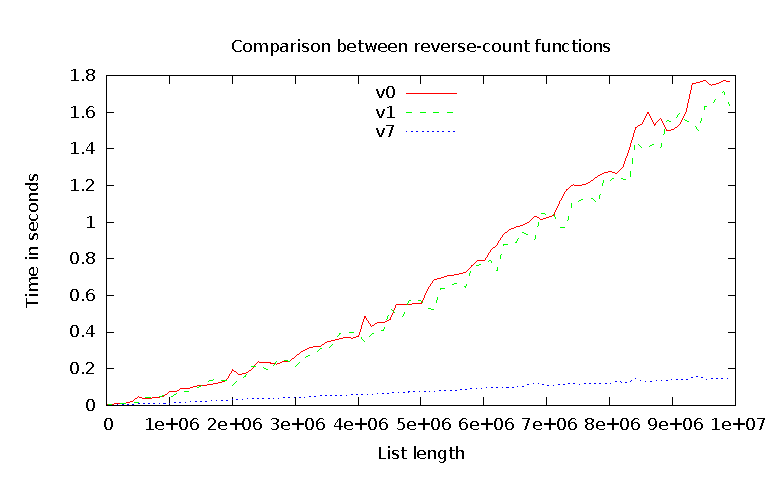
\includegraphics{v0-v1-v7.eps}
\caption{\label{f-versions} Comparison of the behaviour of the three versions on a single system}
\end{figure*}

We see that version \texttt{v7} behaves very well compared the the other two version.
It is not ony faster but also smoother.

%%  LocalWords:  
